\documentclass[lettersize,journal]{IEEEtran} 
\IEEEoverridecommandlockouts
% The preceding line is only needed to identify funding in the first footnote. If that is unneeded, please comment it out.
\usepackage{multirow}%,bigdelim}
\usepackage[hidelinks,draft]{hyperref} % draft is added to bypass issues seen with glossary terms broken up by line-breaks
\newcommand{\emaillink}[1]{\href{mailto:#1}{#1}}
\usepackage{url}
\usepackage{soul}
\usepackage{cite}
\usepackage{amsmath,amssymb,amsfonts}
\usepackage{bm}
\usepackage{mathtools}
\usepackage{siunitx}
\usepackage{xfrac}
% \usepackage{algorithmic}
\usepackage{graphicx}
\graphicspath{{figs/}}
\usepackage{tcolorbox}
\usepackage{textcomp}
\usepackage{xcolor}
\usepackage{siunitx}
\usepackage{xspace}
\usepackage[utf8]{inputenc}
\usepackage{csquotes}
\hyphenation{op-tical net-works semi-conduc-tor IEEE-Xplore}

% \usepackage{tablefootnote}
\usepackage[export]{adjustbox}

% tables
\usepackage{array}
\usepackage{booktabs}
\usepackage{multirow}
\usepackage{makecell}

% Spacing
\usepackage[final]{microtype} % font expansion + protrusion

% \setlist[description]{leftmargin=\parindent,labelindent=\parindent}
\def\BibTeX{{\rm B\kern-.05em{\sc i\kern-.025em b}\kern-.08em
    T\kern-.1667em\lower.7ex\hbox{E}\kern-.125emX}}
% \usepackage[textsize=tiny]{todonotes}
\usepackage[textsize=tiny,disable]{todonotes}
% Maximize margin width to still barely see the sides of todonotes
\setlength{\marginparwidth}{1.3cm}

% Define a todolist for checkboxes
\makeatletter
\let\labelindent\relax
\makeatother
\usepackage[inline]{enumitem}
\newlist{todolist}{itemize}{2}
\setlist[todolist]{label=$\square$}
\usepackage{pifont}
\newcommand{\cmark}{\ding{51}}%
\newcommand{\xmark}{\ding{55}}%
\newcommand{\done}{\rlap{$\square$}{\raisebox{2pt}{\large\hspace{1pt}\cmark}}%
\hspace{-2.5pt}}
\newcommand{\wontfix}{\rlap{$\square$}{\large\hspace{1pt}\xmark}}

% \ifCLASSOPTIONcompsoc
%   \usepackage[caption=false,font=normalsize,labelfont=sf,textfont=sf]{subfig}
% \else
%   \usepackage[caption=false,font=footnotesize]{subfig}
% \fi
\usepackage[caption=false,font=footnotesize]{subfig}
\usepackage{titlecaps}
\usepackage{algorithm,algpseudocode}

%%%%%%%%%%%%%%%%%%%%%%%%%%%%%%%%%%%%%%%%%%%%%%%%%%
% Common macros
%%%%%%%%%%%%%%%%%%%%%%%%%%%%%%%%%%%%%%%%%%%%%%%%%%

\newcommand{\hsia}{H-Si(100)-2$\times$1\@\xspace}
\newcommand{\hsib}{H-Si(111)-1$\times$1\@\xspace}

% referencing labels
\newcommand{\fref}[1]{\figurename~\ref{#1}}
\newcommand{\tref}[1]{\tablename~\ref{#1}}
\newcommand{\secref}[1]{Section~\ref{#1}}
\newcommand{\eref}[1]{Eq.~\eqref{#1}} %\eqref provided by amsmath
\newcommand{\appenref}[1]{Appendix~\ref{#1}}

% in-text functions
\newcommand{\tsps}[1]{\textsuperscript{#1}}  % text superscripts
\newcommand{\tsbs}[1]{\textsubscript{#1}}  % text superscripts
\newcommand{\sref}[1]{\protect\subref{#1}}  % subfig referencing in main caption
\newcommand{\bpar}[1]{(\textbf{#1})}        % bolt text in parentheses

% To-do items
\newcommand{\TODO}[1]{\textcolor{red}{TODO: #1}}
\newcommand{\TODOlow}[1]{\textcolor{blue}{TODO: #1}}
\newcommand{\PLAN}[1]{
    \begin{tcolorbox}[colback=blue!30!white, % Background color
                      colframe=blue!60!black, % Frame color
                      boxsep=1pt, % Box padding
                      arc=2pt, % Corner rounding
                      boxrule=1pt] % Frame thickness
        \tiny
        #1
    \end{tcolorbox}
}
\newcommand{\OLD}[1]{\textcolor{lightgray}{#1}}

% math operators
\DeclareMathOperator\erf{erf}
\DeclarePairedDelimiter\ceil{\lceil}{\rceil}
\DeclarePairedDelimiter\floor{\lfloor}{\rfloor}
\newcommand{\vect}[1]{\boldsymbol{\mathbf{#1}}}
\DeclareSIUnit\angstrom{\text {Å}}

% Terms/math
\newcommand{\etal}{\textit{et al.}}

% \renewcommand{\baselinestretch}{0.99}

% Make \gls output with first letter of each word capitalized, not just first word
% \usepackage{mfirstuc}

\usepackage[acronym]{glossaries}

% Disable hyperlinks for glossary entries
\glsdisablehyper

% ML
\newacronym{ai}{AI}{artificial intelligence}
\newacronym{ml}{ML}{machine learning}
\newacronym{llm}{LLM}{large language model}
\newacronym{qat}{QAT}{quantization-aware training}
\newacronym{api}{API}{application programming interface}

% ML Accel
\newacronym{mvm}{MVM}{matrix--vector multiplication}
\newacronym{mxu}{MXU}{matrix multiply unit}
\newacronym{mac}{MAC}{multiply--accumulate}

% Atomic/Nanotech/Physics
\newacronym{stm}{STM}{scanning tunneling microscope}
\newacronym{afm}{AFM}{atomic force microscope}
\newacronym{set}{SET}{single-electron transistor}
\newacronym{bdl}{BDL}{binary-dot logic}

% Field-Coupled Nanocomputing
\newacronym{fcn}{FCN}{field-coupled nanocomputing}
\newacronym{sidb}{SiDB}{silicon dangling bond}
\newacronym{qca}{QCA}{quantum-dot cellular automata}
\newacronym{nml}{NML}{nanomagnetic logic}

% Devices
\newacronym{hal}{HAL}{hardware abstraction layer}
\newacronym{pi}{PI}{primary-input}
\newacronym{io}{I/O}{input/output}
\newacronym{adc}{ADC}{analog-to-digital converter}
\newacronym{cmos}{CMOS}{complementary metal-oxide-semiconductor}
\newacronym{cad}{CAD}{computer-aided design}
\newacronym{tpu}{TPU}{tensor processing unit}
\newacronym{alu}{ALU}{arithmetic logic unit}

% Architecture
\newacronym{pe}{PE}{processing element}

% EDA
\newacronym{rtl}{RTL}{register-transfer level}
\newacronym{eda}{EDA}{electronic design automation}
\newacronym{aig}{AIG}{And-Inverter Graph}

% fiction-specific algorithms
\newacronym{gold}{\emph{gold}}{graph-oriented layout design}
\newacronym{plo}{\emph{PLO}}{post-layout optimization}

% Others
\newacronym[longplural={figures of merit}]{fom}{FoM}{figure of merit}

\newcommand{\applyalwaysshortacros}{%
  \glsunset{ai}%
  % \glsunset{ml}%
  \glsunset{llm}%
  \glsunset{cmos}%
  \glsunset{cad}%
}

\applyalwaysshortacros

% solve error: Page 1 has margin impositions
\def\IEEEtitletopspace{18pt}

\clubpenalty = 10000
\widowpenalty = 10000
\displaywidowpenalty = 10000

\begin{document}

\title{RTL-to-Atoms Synthesis of a Machine Learning Accelerator on Atomic-Scale Computers}

% \author{Anonymous author(s)}
\author{%
    Samuel~S.~H.~Ng, %
    Marcel Walter, %
    Simon Hofmann, %
    Jan Drewniok, %
    Robert Wille, %
    and Konrad Walus%
    % \thanks{This work was supported by the Natural Sciences and Engineering Research Council of Canada under Grant \mbox{RGPIN-2022-04830}.}%
    \thanks{S.~Ng and K.~Walus were with the Department of Electrical and Computer Engineering, University of British Columbia, Canada (\{\mbox{samueln}, \mbox{konradw}\}@ece.ubc.ca); M.~Walter, S.~Hofmann, J.~Drewniok, and R.~Wille were with the Chair for Design Automation, Technical University of Munich, Germany (\{\mbox{marcel.walter}, \mbox{simon.t.hofmann}, \mbox{jan.drewniok}, \mbox{robert.wille}\}@tum.de). M.~Walter, S.~Hofmann, and R.~Wille were also with the Munich Quantum Software Company GmbH, Germany. R.~Wille was also with the Software Competence Center Hagenberg (SCCH) GmbH, Austria.}%
}

% \section*{Extension Plan}

% \subsection*{Main objectives}

% Objectives that, together, satisfy \SI{50}{\percent} new contents rule:
% %
% \begin{todolist}
%     \item[\done] Implement ripple-carry adder and array multiplier in Verilog with a wrapper that automatically generates N-bit versions
%     \item[\done] Testbench the above for verification
%     \item[\done] In the Processing Element, replace multiplication and accumulation operations with the optimized \glspl{alu} \textcolor{orange}{using Yosys's technology mapper}
%     \item[\done] Synthesize and report changes
%     \item \textcolor{orange}{Post-Yosys equivalence check (use PE-forward test bench)}
%     \item[\done] \textcolor{orange}{Extend Verilogs to accept arbitrary width and activation bit-width settings}
%     \item New table similar to DATE's table: report multiple algorithm combinations (e.g., ortho with and without PLO, FoM vs. uniform gates), \textcolor{orange}{test multiple bit-widths (W8A8, W4A4, W2A2)}, report FoM-informed results similarly
%     \begin{itemize}
%         \item Further study possible with gold with different cost metrics (e.g., area vs crossing vs area-crossing product etc.)
%         \item Using CP as cost function might give us more squarish outputs
%     \end{itemize}
% \end{todolist}

% \subsection*{Stretch goals}

% \begin{todolist}
%     \item Add half-adder gate to technology mapper
%     \begin{itemize}
%         \item \textcolor{orange}{Simon to look into adding HA to TM and synthesizing via \emph{gold}}
%         \item \textcolor{orange}{Highly good-to-have if achievable without major roadblocks, do not sink too much time if there are significant hurdles!}
%     \end{itemize}
%     % \item \textcolor{red}{Demoted from main objectives:} Create multi-attempt averaged score benchmark set:
%     % \begin{itemize}
%     %     \item To clarify, this is an attempt at realizing that ``scientifically rigorous'' synthesis results comparison
%     %     \item We can create a long-running script that makes $N$ attempts at deepsyn, TM to FoM-informed and uniform gates, $M$ attempts at \emph{gold} (if tractable). Since \emph{PLO} is deterministic we won't have to rerun that. This means $2 \cdot N \cdot M$ attempts in total. Missing anything?
%     % \end{itemize}
%     % \item If there's time, also try to improve the pin-routing area estimation (either by hand or by auto routing if available)
%     % \begin{itemize}
%     %     \item Marcel: can try using color routing in fiction
%     %     \item Alternatively, Ben's planar placement \& routing algorithm
%     % \end{itemize}
% \end{todolist}


\maketitle

\begin{abstract}
%
As \gls{cmos} scaling slows and \gls{ai} demand soars, atomic-scale platforms such as quantum-dot logic based on \glspl{sidb} offer a promising path toward energy-efficient computation, yet practical design flows from \gls{rtl} specifications to manufacturable layouts remain limited.
This work presents an \gls{rtl}-to-atoms synthesis framework for a quantized \glsentrylong{mxu} targeting \gls{sidb}-based \gls{fcn}.
Building on recent advances in \gls{sidb}-aware \gls{eda}, the framework combines a hierarchical, parameterized \gls{rtl} architecture with platform-optimized \glsentrylongpl{alu}, reducing the synthesized logic core of processing elements by about $\bm{15\,\%}$ compared to prior flows.
Key improvements were also made to the synthesis workflow, retargeting tools previously tuned for other \gls{fcn} technologies\todo{Sam to Marcel: do you think this is clearer? Original comment was ``what was it optimized to before?''} toward \gls{sidb} logic and incorporating figure-of-merit awareness, which together ensure that the synthesized layouts achieve favorable area scaling and maximum throughput while balancing operational robustness.
Evaluations across multiple quantization bit-widths show substantial footprint reductions for configurations within the practical range of latest placement-and-routing algorithms while preserving testbench-validated functional correctness from \gls{rtl} to dot-accurate \gls{sidb} layouts, thereby establishing a reproducible benchmark for \gls{eda} on atomic-scale computing.
This represents a significant milestone, bridging previously manually-intensive workflows with scalable, automated methodologies, thus providing a valuable foundation for future design and optimization of \gls{sidb}-based accelerators.
%
\end{abstract}

% \begin{IEEEkeywords}
% Computer aided design, machine learning acceleration, quantum dots, silicon dangling bonds, simulation
% \end{IEEEkeywords}


\glsresetall
\applyalwaysshortacros

%%%%%%%%%%%%%%%%%%%%%%%%%%%%%%%%%%%%%%%%%%%%%%%%%%
% Introduction
%%%%%%%%%%%%%%%%%%%%%%%%%%%%%%%%%%%%%%%%%%%%%%%%%%
\section{Introduction} \label{sec:intro}

\IEEEPARstart{G}{lobal} computing infrastructure increasingly devotes its resources to \gls{ai} inference and training, making the associated energy demand a central constraint and spurring efforts to develop hardware platforms that operate far more efficiently than traditional \gls{cmos} processors.
Among these, \gls{fcn} has emerged as an appealing post-\gls{cmos} computing paradigm, in which local field interactions encode logic states in the position of charges~\cite{lent2003molecular} or in the magnetic polarity of nanomagnets~\cite{bernstein2005magnetic,giri2016modeling}, enabling both computation and signal transmission.

Among the various physical implementations of \gls{fcn}, quantum dots made of \glspl{sidb} stand out as a promising platform due to their atomically precise fabrication~\cite{achal2018lithography, pitters2024atomically} and discretely controllable charge states~\cite{haider2009controlled, pitters2011charge}.
Motivated by the experimental demonstration of an \gls{sidb} \textsc{or} gate measuring just $\SI{5}{\nano\meter}\times\SI{6}{\nano\meter}$~\cite{huff2018binary}, specialized \gls{cad} tools and \gls{eda} frameworks have emerged to support \gls{sidb} logic exploration.
At the physical design level, \emph{SiQAD}~\cite{ng2020siqad} and an ecosystem of simulators~\cite{chiu2020poissolver,drewniok2024need,lambooy2026clustercomplete} have enabled the exploration of logic structures and design rules at the gate and circuit levels~\cite{vieira2022threeinput,ruella2025comprehensive}.
However, the fully manual design of these layouts remained a time-consuming process, motivating the automation of multiple stages of the design flow. At the quantum-dot level, automated \gls{sidb} gate designers~\cite{drewniok2025quickcell} enabled the creation of standard-tile libraries~\cite{walter2022hexagons}. With the addition of \gls{sidb} support in \emph{fiction}~\cite{walter2019fiction}, an \gls{eda} framework specialized for \gls{fcn}, new pathways have been opened for large-scale designs by synthesizing gate-level netlists down to dot-accurate \gls{sidb} layouts.

Prior to the maturity of \gls{sidb} \gls{eda} tools, application-scale research targeting \glspl{sidb} was scarce and relied on manually verified \gls{sidb} building blocks, which were then extrapolated into system-level designs to estimate their behavior and implementation costs \cite{chiu2020poissolver, ng2023blueprint}. Among them was a quantized \gls{mxu} inspired by Google's \gls{tpu}~\cite{jouppi2017indatacenter} and optimized for \gls{sidb}'s architectural constraints~\cite{ng2023blueprint}, where simulation-proven \gls{sidb} logic components were used to approximate the area cost and performance figures.
To facilitate practical exploration, an earlier conference version of this work~\cite{ng2025building} implemented the \gls{mxu} as a \gls{rtl} Verilog design, employing clocked registers as an abstract proxy for the underlying \gls{fcn} clocking behavior. With a workflow spanning multiple \gls{eda} frameworks, the study synthesized the \gls{rtl} implementation into dot-accurate \gls{sidb} layouts, realizing an automated, scalable, and verifiable end-to-end \gls{sidb} design flow using state-of-the-art \gls{eda} tools.

Despite this progress, the conference version of the \gls{rtl}-to-atoms flow in~\cite{ng2025building} left several aspects only coarsely explored: the choice of \glspl{alu} was left to logic synthesis frameworks, which do not take \gls{fcn}'s unique architectural preferences into account. Weights and activations were fixed to a single 8-bit configuration, preventing systematic study of how the synthesized layouts scale with precision.
This work therefore provides a substantial extension upon the original methodology at multiple layers: at the \gls{rtl} design layer, parameterized quantization enabled a systematic study of downstream trade-offs in the synthesis pipeline; for \gls{rtl}-to-netlist synthesis, the introduction of technology-appropriate \glspl{alu} reduced the resulting area; and for netlist-to-atoms synthesis, multiple \gls{sidb}-oriented refinements to technology mapping, placement-and-routing, and hexagonalization further had a significant impact on the quality of result.
These contributions transform a one-off demonstration into a concrete framework optimized for \gls{sidb} logic synthesis, revealing how architectural and layout decisions shape the strengths and limitations of current tools.
The remainder of this manuscript is structured as follows: \secref{sec:background} reviews \gls{sidb} logic background and \gls{eda} infrastructure; \secref{sec:related-work} summarizes prior \gls{sidb} \gls{mxu} designs; \secref{sec:methodology} details the hierarchical \gls{rtl} architecture and the \gls{rtl}-to-atoms synthesis flow; \secref{sec:results} presents the synthesis results and discuss their trade-offs; and \secref{sec:conclusion-future-work} concludes with directions for future work.

%%%%%%%%%%%%%%%%%%%%%%%%%%%%%%%%%%%%%%%%%%%%%%%%%%
% Background
%%%%%%%%%%%%%%%%%%%%%%%%%%%%%%%%%%%%%%%%%%%%%%%%%%
\section{Background} \label{sec:background}

\begin{figure}
    \centering
    \subfloat[\gls{sidb} unit cell.]{
        \includegraphics[width=.25\linewidth,valign=c]{figs/bdl_demo.pdf}
        \label{sfig:sidb-logic-pairs}
    }\quad
    \subfloat[\emph{Bestagon} \textsc{nand} gate.]{
        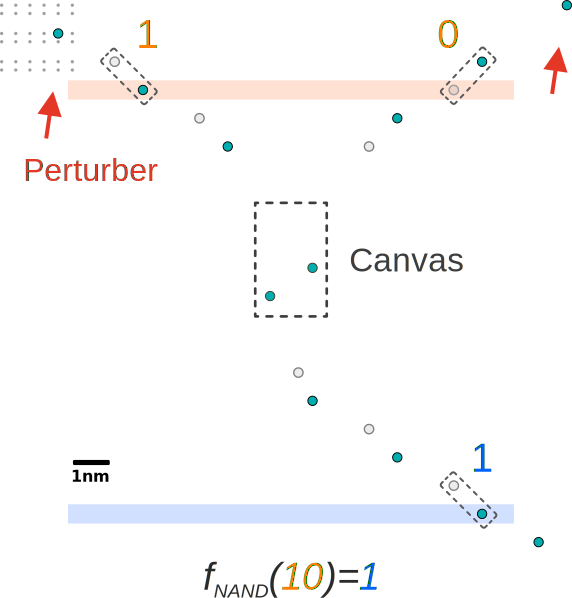
\includegraphics[width=.55\linewidth,valign=c]{figs/nand_10_bestagon_gate.pdf}
        \label{sfig:sidb-logic-hex-tile}
    }
    \caption{
        (\textbf{a}) \gls{sidb} logic unit cell: a pair of closely-spaced \glspl{sidb} share a charge whose position encodes logic \texttt{0} or \texttt{1}, controlled by the location of a nearby \enquote{perturber} \gls{sidb}.
        (\textbf{b}) Example \textsc{nand} gate from the \emph{Bestagon} library, with inputs applied at the upper pins via perturbers, and the output sensed at the lower pin; the central region hosts \glspl{sidb} that implement the gate function. With permission, (a) is reproduced from~\cite{ng2023blueprint}, (b) is adapted from~\cite{drewniok2025quicktrace}.
    }
    \label{fig:sidb-logic}
\end{figure}



\Glspl{sidb} can be fabricated on the surface of hydrogen-passivated Si(100)-2$\times$1 with the tip of a scanning-tunneling microscope \cite{achal2018lithography,pitters2024atomically}. Each \gls{sidb} can hold discrete charge states, including negative, neutral, or positive. In densely packed ensembles, the charge state of each \gls{sidb} is determined by their collective interaction, bulk doping levels, and external electrostatic influences~\cite{pitters2024atomically}.
Binary logic states can be encoded by the position of a charge shared among closely positioned \glspl{sidb} (\fref{sfig:sidb-logic-pairs}), enabling the experimental demonstration of an \textsc{or} gate with a footprint of only $5\times\SI{6}{\nm^2}$~\cite{huff2018binary}.
Further exploration of \gls{sidb} logic designs was enabled by \emph{SiQAD}~\cite{ng2020siqad}, a \gls{cad} tool specialized for \gls{sidb} logic. Building on these tools, the \emph{Bestagon} standard-tile library~\cite{walter2022hexagons} was introduced, featuring standardized \gls{io} pin locations and a central canvas on which \glspl{sidb} are placed to implement logic (\fref{sfig:sidb-logic-hex-tile}).
The \emph{Bestagon} library has allowed \emph{fiction}~\cite{walter2019fiction}, an \gls{eda} framework specialized for \gls{fcn}, to take gate-level netlists as input and synthesize dot-accurate, fabricable \gls{sidb} layouts~\cite{walter2022hexagons}, forming the backbone of this work.

\Gls{sidb} logic, like other \gls{fcn} families, uses spatially partitioned clock zones to enforce directed data flow~\cite{ng2020siqad, chiu2020poissolver}. Hanging or buried electrodes apply phase-shifted sinusoidal potentials that modulate the surface band bending and thereby the local charge density~\cite{chiu2020poissolver}. Adjacent electrodes are offset by \SI{90}{\degree} in phase, producing \enquote{active} regions where charges are present, and computation occurs, separated by \enquote{inactive} regions that are effectively charge-free buffers. An area-efficient arrangement places these clock zones in rows to support unidirectional, purely combinational logic~\cite{lent1997device,chiu2020poissolver}.
Interfacing with \gls{cmos} can be achieved by biasing inputs electrostatically via electrodes~\cite{chiu2020poissolver}, while outputs can be sensed using charge-sensitive devices such as single-electron transistors~\cite{fuechsle2012singleatom, prager2009integration, bohloul2017quantum}.

%%%%%%%%%%%%%%%%%%%%%%%%%%%%%%%%%%%%%%%%%%%%%%%%%%
% Related work
%%%%%%%%%%%%%%%%%%%%%%%%%%%%%%%%%%%%%%%%%%%%%%%%%%
\section{Related Work} \label{sec:related-work}

In this section, \secref{sec:related-work-fcn-eda} surveys existing \gls{fcn} \gls{eda} frameworks, and \secref{sec:related-work-sidb-ml-accel} reviews \gls{sidb} \gls{mxu} designs. Together, they contextualize the proposed \gls{rtl}-to-atoms flow.

\subsection{Electronic Design Automation for FCN}\label{sec:related-work-fcn-eda}

Aside from \emph{fiction}, other \gls{fcn} \gls{eda} frameworks target \gls{nml}, a field-coupled style in which information is stored and propagated via the collective magnetization of interacting nanomagnets rather than mobile charges.\todo{Sam to Marcel: in light of your comment that NML could better be introduced in sections 1 or 2, I made a few attempts and didn't land on a clean/punchy narrative without adding too much text. So I've instead resorted to adding an inline introduction here, hope it works.}
Within this setting, \emph{ToPoliNano}~\cite{riente2017topolinano} provides a top-down flow from structural VHDL descriptions to in-plane \gls{nml} layouts with clocking-aware placement and routing.
Complementing this, \emph{FUNCODE}~\cite{garlando2021funcode} infers VHDL netlists from custom \gls{nml} layouts, enabling device-to-system analysis of \gls{nml} circuits using HDL simulators.
These works demonstrate \gls{fcn} \gls{cad} capabilities in the \gls{nml} domain.
In contrast, the present work targets the emerging atomic-scale \gls{sidb} logic platform, for which \gls{rtl}-to-atoms design flows are maturing.

\begin{figure}
    \centering
    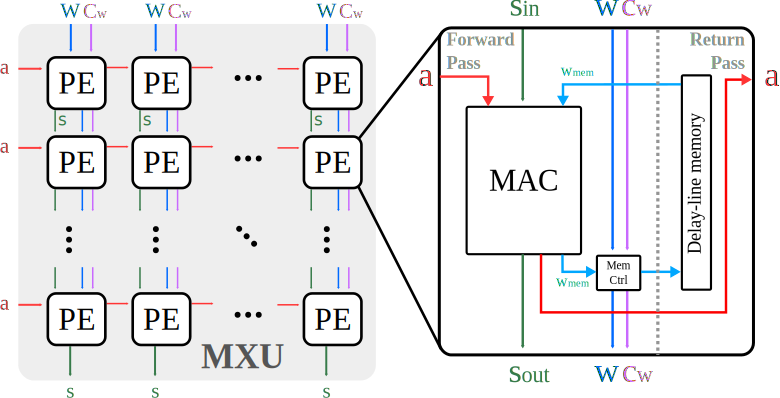
\includegraphics[width=0.95\linewidth]{figs/mxu_sa_colored.pdf}
    \caption{
        A 2D systolic array \glsentryshort{mxu} receiving quantized activations $a$, weights $w$, control signals $c_w$, and partial sums $s$. Each \glsentryshort{pe} consists of a \glsentryshort{mac} unit, memory controller, and memory for weight storage. Signals propagate downward on the left (forward pass) and upwards on the right (return pass).
        % \TODO{Consistent font size \& weight for I/O pins.} \TODO{Improve color scheme.} \TODO{Rounded corners in the right.}
        % \TODO{Simon: Is the capitalization of w and c consistent? For example its C in the left figure and c in the right (also regarding the caption)}
    }
    \label{fig:mxu-systolic-array}
\end{figure}

\subsection{SiDB ML Accelerators}\label{sec:related-work-sidb-ml-accel}

Before dedicated \gls{sidb}-aware \gls{eda} tooling became available, studies of \gls{sidb} applications were limited and largely depended on manual \gls{cad} prototyping with extrapolated area and latency estimates.
One such example was an \gls{sidb} \gls{mxu}~\cite{ng2023blueprint} for \gls{ml} acceleration, which mirrored design choices from Google's \gls{tpu}v1~\cite{jouppi2017indatacenter}: the matrix-vector multiplications underpinning \gls{ml} workloads were realized as 8-bit integer \gls{mac} operations to reduce computational cost, and both designs employed a systolic-array architecture relying on regular arrangements of \glspl{pe}---homogeneous logic modules that operate on their inputs and pass results to adjacent \glspl{pe}---to perform computation (\fref{fig:mxu-systolic-array}).
At the \gls{pe} level, the core operation is a \gls{mac}: $s_{\text{out}} = s_{\text{in}} + (w \cdot a)$, where $s_\text{in}$ the partial sum from the preceding \gls{pe}, $w$ is the stored weight, $a$ is the activation, and $s_\text{out}$ is the updated partial sum.

In the implementation of~\cite{ng2023blueprint}, each matrix-multiplication job consisted of two primary phases:
%
\begin{enumerate*}
  \item \emph{preloading}, where weights ($w$) are loaded into the array from the top edge and traverse column-wise until they arrive at the designated \glspl{pe} for storage;
  \item \emph{computing}, where activations ($a$) are streamed from the left side and are multiplied with the stored weights and accumulated with partial sums; activations continue to traverse row-wise while partial sums traverse column-wise for further accumulation until they reach the array's bottom edge.
\end{enumerate*}
%
Additional input signals control the operating phase.
At the \gls{pe} granularity, each \gls{pe} comprises two signal paths: a \emph{forward pass} containing the \gls{mac} and memory controller, and a \emph{return pass} that drives a weight bus upward to close the delay-line memory feedback loop and an activation bus to align activations with neighboring \glspl{pe} (\fref{fig:mxu-systolic-array}). Both paths are purely combinational, enabling row-wise clocking on each path.
Row-wise clocking incurs deep pipeline stages, which can be taken advantage of by interleaving different inputs by clock cycle to increase the computational throughput.


While that blueprint study reported promising area and power estimates against the \gls{tpu}v1~\cite{ng2023blueprint, jouppi2017indatacenter}, its extrapolated nature offered neither a manufacturable layout nor formal verification. The preceding conference version of this work~\cite{ng2025building} bridged this gap by applying latest \gls{sidb} \gls{eda} techniques to demonstrate a \gls{rtl}-to-atoms synthesis flow to a quantized \gls{sidb} \gls{mxu}, which this work substantially refines by introducing technology-specific optimizations and exploring the scaling behavior of different quantization bit-widths, as detailed in the next section.

%%%%%%%%%%%%%%%%%%%%%%%%%%%%%%%%%%%%%%%%%%%%%%%%%%
% Methodology
%%%%%%%%%%%%%%%%%%%%%%%%%%%%%%%%%%%%%%%%%%%%%%%%%%
\section{Proposed Methodology} \label{sec:methodology}

This section presents the proposed end-to-end \gls{rtl}-to-atoms design and synthesis flow.
\secref{sec:methodology-verilog} describes the hierarchical \gls{rtl} architecture at the core of the flow, which satisfies tooling requirements.
Subsequently, \secref{sec:methodology-rtl-to-netlist} covers the \gls{rtl}-to-netlist conversion, and \secref{sec:methodology-netlist-to-atoms} describes the netlist-to-atoms physical design with optimizations for \glspl{sidb}.

\subsection{\titlecap{\glsentrylong{mxu}} in Hierarchical RTL}\label{sec:methodology-verilog}

\begin{algorithm}[tbp]
\footnotesize
\caption{Forward Pass Logic in Processing Element}\label{alg:pe-forward}

\renewcommand{\algorithmicrequire}{\textbf{Inputs:}}
\renewcommand{\algorithmicensure}{\textbf{Outputs:}}

\begin{algorithmic}[1]
    \newcommand{\codecomment}[1]{\textit{\textcolor{gray}{// #1}}}
    \Require
    \Statex $\mathit{PE}_{y} \gets$ y-index assigned to each PE (constant per PE)
    \Statex $m \gets$ PRELOAD (0) or COMPUTE (1) mode
    \Statex $w_\text{load} \gets$ weight to be loaded into memory
    \Statex $\mathit{PE}_{\text{target-}y} \gets$ target Y-index of $w_\text{load}$
    \Statex $s_\text{in} \gets$ input partial product
    \Statex $a \gets$ input activation
    \Statex $w_\text{mem} \gets$ weight loaded from delay-line memory

    \Ensure
    \Statex $s_\text{out}$: new partial sum
    \Statex $w_\text{memOut}$: weight to write to delay-line memory

    \Procedure{ProcessingElementLogic}{}
    \State $p \gets \text{signed}(w_\text{mem}) \times \text{signed}(a)$\Comment{Multiply stored $w$ with $a$}
    \State $s_\text{out} \gets s_\text{in} + \text{signExtend}(p, 24)$\Comment{Sum with partial sum}
    \If{$m = \text{PRELOAD}$ \textbf{and} $\mathit{PE}_{\text{target-}y} = \mathit{PE}_{y}$}
       \State $w_\text{memOut} \gets w_\text{load}$\Comment{Update stored weight}
    \EndIf
    \State \Return $s_\text{out}$, $w_\text{memOut}$, and other pass-through wires
    \EndProcedure
\end{algorithmic}
\end{algorithm}

To achieve this work's objectives, the \gls{rtl} implementation must satisfy the following requirements:
%
\begin{enumerate*}
  \item the \gls{rtl} must be purely combinational for \emph{fiction} compatibility; and
  \item operation of the pipelined \gls{pe} must be verifiable so that test benches can establish operational correctness, addressing the lack of formal verification in prior work~\cite{ng2023blueprint}.
\end{enumerate*}
%
Because the \gls{pe} includes forward and return paths that form an internal feedback loop, a direct \gls{rtl} implementation of the full \gls{pe} would be incompatible with \emph{fiction}.
In reconciliation, this work adopts a hierarchical \gls{rtl} organization which compartmentalizes the design:
%
\begin{description}
  \item[Combinational core:] The \gls{pe}'s forward-pass logic is implemented in strictly combinational \gls{rtl}, as shown in Alg.~\ref{alg:pe-forward}, ensuring compatibility with subsequent synthesis steps.
  \item[Clocked shell:] A higher-level \gls{rtl} module captures the clocked operation of the full \gls{pe}, defining the component's input and output signals, pipelined internal signal steering, and synchronized signal timing for the return pass.
\end{description}
%
Both are parameterized by the weight and activation bit-widths, allowing the study of their scaling behavior in \secref{sec:results}.

Correctness was validated with test benches across both layers. These tests confirmed correct weight storage in preload mode and accurate \gls{mac} results in compute mode for representative inputs.
In particular, interleaved inputs for concurrent \gls{mac} operation across all pipeline stages was also verified. All simulations were performed using Icarus Verilog~\cite{icarusverilog}, establishing logical correctness of the \gls{pe} prior to synthesis and physical mapping. The codebase is fully open sourced.\footnote{GitHub repository: \url{https://github.com/samuelshng/sidb-mxu-verilog}}

\subsection{RTL-to-Netlist}\label{sec:methodology-rtl-to-netlist}


With the \gls{rtl} design verified, the first stage of the synthesis flow is to generate a gate-level netlist. To accomplish this, this work uses \emph{Yosys}~\cite{wolf2013yosys} to map arithmetic operators such as \mbox{accumulation (\texttt{+})} and \mbox{multiplication (\texttt{*})} into gate-level \glspl{alu}.
Absent explicit directives, \emph{Yosys} selects \gls{cmos}-optimized \glspl{alu}, which underperform in \gls{fcn} due to differences in area and latency trade-offs under the strictly planar fabric~\cite{kim2010multipliers}.
To ensure technology-appropriate choices, this work supplies explicit gate-level descriptions of a ripple-carry adder and an array multiplier to \emph{Yosys}, both of which have been shown to be suitable for \gls{fcn} thanks to their regular structure, which eases wiring congestion \cite{kim2010multipliers}.
The mapped netlist is then rewritten as an \gls{aig} and optimized with ABC's \textit{\&deepsyn}~\cite{brayton2010abc} strategy to reduce its node count, and re-validated against test benches to confirm functional correctness.

\subsection{Netlist-to-Atoms}\label{sec:methodology-netlist-to-atoms}

The optimized \gls{aig} is then passed to \emph{fiction} for the second stage of the synthesis flow: physical design. This stage transforms the netlist into a dot-accurate \gls{sidb} layout through a multi-step process, which this work enhances with several optimizations for the \gls{sidb} platform.

\subsubsection{Synthesis Flow}

% The verified \gls{aig} is subsequently forwarded to \emph{fiction}, whose \gls{fcn}-aware toolchain synthesizes it into an \gls{sidb} layout following the synthesis flow proposed by \cite{walter2022hexagons}:

This work starts with the \gls{sidb}-specific flow in \emph{fiction} proposed by \cite{walter2022hexagons}:
%
\begin{description}
  \item[Technology mapping] maps the \gls{aig} onto the \emph{Bestagon} gate library~\cite{walter2022hexagons}, exploiting the library's richer primitives to shrink the logic compared with an AND/INV-only basis.
  \item[Placement and routing] with the \textit{ortho}~\cite{walter2019scalable} or \gls{gold}~\cite{hofmann2025graphoriented} algorithm produces a layout on a Cartesian grid.
  \item[\Gls{plo}~\cite{hofmann2025efficient}] reduces the footprint of the routed design.
  \item[Hexagonalization] projects the Cartesian layout onto a hexagonal grid~\cite{hofmann2023scalable} to align with \emph{Bestagon} gates.
  \item[SAT-based equivalence checking~\cite{walter2020verification}] confirms that the hexagonalized layout preserves the gate-level behavior.
  \item[Atom mapping] maps each tile in the verified layout to the corresponding \emph{Bestagon} gate's \gls{sidb} arrangement, yielding a dot-accurate, manufacturable \gls{sidb} layout.
\end{description}
%
While this established workflow provides a robust foundation, its application to the \gls{sidb} platform revealed opportunities for technology-specific enhancements as detailed below.

\subsubsection{FoM-aware Technology Mapping}

Previous \gls{sidb} synthesis flows within \emph{fiction} treated all gates in the technology library as equivalent, without physical robustness considerations.
Recent \gls{sidb} logic robustness studies have culminated in the creation of a unified cost function for \glspl{fom}~\cite{drewniok2024unifying}. The cost function encompasses the dominant cost drivers---operational domain size~\cite{ng2020siqad, walter2023reducing}, thermal stability~\cite{drewniok2023temperature}, band-bending effects~\cite{pitters2011charge}, defect sensitivity~\cite{ng2024simulating}, and related factors---into a single \gls{fom}.
This work adopts it as the objective for the technology mapper to prioritize gates with higher predicted robustness, accepting a potential trade-off in other layout metrics like area or quantum-dot count.

\subsubsection{Placement and Routing Optimizations}\label{subsubsec:methodology-p-and-r-improvements-for-sidb}

The placement-and-routing framework within \emph{fiction} was first established for \gls{qca} circuits on a Cartesian grid~\cite{walter2019fiction}\todo{Sam to Marcel: I removed 2DDWave mention here altogether because the clocking scheme only really becomes more important in the Hexagonalization subsec}. Subsequent support for \gls{sidb} logic was enabled through a coordinate mapping that performs a $45^\circ$ rotation of the Cartesian layout followed by its projection onto the hexagonal \gls{sidb} lattice~\cite{hofmann2023scalable}.
This rotation, however, can lead to suboptimal results: a layout that is compact on the Cartesian grid may become significantly taller after hexagonalization when there exists numerous diagonal signal paths in the Cartesian layout that are strongly offset from the northwest corner, which map to long vertical paths in the hexagonal layout. Layouts with a more balanced aspect ratio are therefore preferred.
While the older \emph{ortho} algorithm offers no configurable compensation, the more recent \gls{gold} algorithm~\cite{hofmann2025graphoriented} exposes a customizable cost objective for placement and routing, enabling \gls{sidb}-specific optimizations.
Whereas the default cost objective for \gls{gold} is the total area, this work introduces new cost objectives that reduce the aspect-ratio distortion introduced by the $45^\circ$ rotation by encouraging more square footprints, which is further detailed in \secref{sec:results-synthesis-metrics}.

\subsubsection{Hexagonalization Improvements}

The hexagonalization algorithm was also revised in this work to align generated layouts with \gls{sidb} clocking expectations. Under the Cartesian layout's 2DDWave clocking scheme~\cite{vankamamidi2008twodimensional}, primary inputs are placed along the north and west borders, and data advances diagonally toward the southeast. The $45^\circ$ rotation left many \gls{io} pins recessed from the north and south edges, which reduces the attainable throughput because some signals must be held across multiple cycles for synchronization. The updated flow stretches all \gls{io} pins to the north and south boundaries after projection, producing layouts whose ports are time-aligned as they enter and exit the hexagonal fabric. An optional constraint can be toggled to perform the pin extensions without wire crossings as they are typically less robust against environmental defects.

%%%%%%%%%%%%%%%%%%%%%%%%%%%%%%%%%%%%%%%%%%%%%%%%%%
% Experiments
%%%%%%%%%%%%%%%%%%%%%%%%%%%%%%%%%%%%%%%%%%%%%%%%%%
\section{Experiments}\label{sec:results}

This section evaluates the \gls{rtl}-to-atoms flow using the synthesized \gls{pe}-core layouts.
\secref{sec:results-experimental-protocol} outlines the experimental protocol and configurations.
\secref{sec:results-synthesis-metrics} presents the resulting synthesis metrics across technology-mapping and placement-and-routing variants.
\secref{sec:results-discussion} discusses these findings and compares them with prior manual estimations.

\subsection{Experimental Protocol}\label{sec:results-experimental-protocol}

This comparative study characterizes how activation and weight bit-widths scale and reports synthesis results across various synthesis configurations.
To this end, the combinational \gls{pe}-core (\secref{sec:methodology-verilog}) is synthesized for 2-, 4-, and 8-bit weights and activations, henceforth denoted W2A2, W4A4, and W8A8, respectively.
These selections correspond to widely studied quantized regimes for  \gls{ml} workloads where the dominant operations reduce to dense matrix multiplications~\cite{esser2020learnedstepsizequantization,banner2019post,jouppi2017indatacenter}.
The \gls{rtl}-to-netlist flow from this work instructs \emph{Yosys} to use technology-appropriate \glspl{alu} to produce an \gls{aig} (\secref{sec:methodology-rtl-to-netlist}), which is then optimized using ABC's \emph{\&deepsyn} strategy~\cite{brayton2010abc}. %On a AMD Ryzen 9 3900X CPU, \emph{\&deepsyn} reached its internal iteration limit at \SI{0.4}{\hour}, \SI{1}{\hour}, and \TODO{} for W2A2, W4A4, and W8A8, respectively.
In the netlist-to-atoms flow, two \emph{Bestagon} library~\cite{walter2022hexagons} variants are compared during technology mapping: a uniform cost baseline, and an \gls{fom}-aware counterpart. \emph{ortho} and \gls{gold} are used for placement and routing.

\subsection{Results}\label{sec:results-synthesis-metrics}

\begin{table}
  \caption{Synthesis comparison across \gls{mxu} and \gls{eda} configurations}
  \centering
  \label{tab:pe-results-extended}
  \begin{minipage}{\linewidth}
    \centering
    \begin{tabular}{l@{\hskip 6pt}l@{\hskip 6pt}l@{\hskip 6pt}
                    r@{~$\times$~}l@{~$=$~}r@{\hskip 12pt}
                    r}
      \toprule
      \multirow[c]{2}{*}{\makecell[tl]{\textsc{\glspl{alu}}}} &
      \multirow[c]{2}{*}{\makecell[tl]{\textsc{PE}}} &
      \multirow[c]{2}{*}{\makecell[tl]{\textsc{Alg}}} &
      \multicolumn{3}{c}{\textsc{Uniform TM}} &
      \multirow[c]{2}{*}{\makecell[tl]{$A_\text{FoM}$}} \\
      % \textsc{FoM-aware TM} \\
      \cmidrule(lr{12pt}){4-6}
        & & & $w$ & $h$ & $A_\text{uni}$ & \\
      \midrule
      Default~\cite{ng2025building} & W8A8 & \emph{ortho}+\gls{plo} &
      \num{515} & \num{1043} & \num{537145} &
      \num{541284} \\
      \cmidrule(lr){1-7}
      \multirow[t]{5}{*}{\makecell[tl]{Optimized\\(This work)}} & W8A8 & \emph{ortho}+\gls{plo} &
      \num{474} & \num{967} & \num{458358} &
      \num{470830} \\[0.8ex]
        & \multirow[t]{2}{*}{W4A4} & \emph{ortho}+\gls{plo} &
      \num{143} & \num{333} & \num{47619} &
      \num{56744} \\
        &  & \emph{gold}+\gls{plo} &
      \num{116} & \num{241} & \num{27956} &
      \num{70070} \\[0.8ex]
        & \multirow[t]{2}{*}{W2A2} & \emph{ortho}+\gls{plo} &
      \num{67} & \num{151} & \num{10117} &
      \num{10833} \\
        &  & \emph{gold}+\gls{plo} &
      \num{48} & \num{98} & \num{4704} &
      \num{5457} \\
      \bottomrule
    \end{tabular}
    \begin{minipage}{\linewidth}
      \footnotesize
      \vspace{0.5em}
      \enquote{Default} and \enquote{optimized} \glspl{alu} indicate \emph{Yosys}'s \gls{alu} selection mode; $w$ and $h$ denote the tile counts along the width and height; $A = w \times h$; $A_\text{uni}$ and $A_\text{FoM}$ denote the \emph{Bestagon} variant used for technology mapping.  %\TODO{Do a final check with sweep data to make sure the reported minimums accurately reflect latest results.}
      % \gls{plo} was used together with each algorithm.
    \end{minipage}
  \end{minipage}
\end{table}

\begin{table}
  \caption{Cost objective comparison for \emph{gold} algorithm}
  \centering
  \label{tab:gold-cost-comparison}
  \begin{minipage}{\linewidth}
    \centering
      \begin{tabular}{l@{\hskip 4pt}l@{\hskip 8pt}
                      r@{\hskip 3pt}r@{\hskip 8pt}
                      r@{\hskip 3pt}r}
        \toprule
        \textsc{PE} &
        \textsc{Cost obj} &
        \multicolumn{2}{l}{$A_\mathrm{min}$} &
        \multicolumn{2}{l}{$\bar{A}$} \\
        \midrule
        \multirow[t]{3}{*}{\makecell[tl]{W4A4}} & Area (baseline) &
        \num{27956} &  &
        \num{37483.61} & \\
         & $x + y$ &
        \num{27956} & $(+\SI{0.00}{\percent})$ &
        \num{37303.28} & $(\SI{-0.48}{\percent})$ \\
         & $x^{2} + y^{2}$ &
        \num{28175} & $(+\SI{0.78}{\percent})$ &
        \num{36716.71} & $(\SI{-2.05}{\percent})$ \\
        \cmidrule(lr){1-6}
        \multirow[t]{3}{*}{\makecell[tl]{W2A2}} & Area (baseline) &
        \num{5145} & &
        \num{10156.22} & \\
         & $x + y$ &
        \num{5145} & $(+\SI{0.00}{\percent})$ &
        \num{8107.02} & $(\SI{-20.18}{\percent})$ \\
         & $x^{2} + y^{2}$ &
        \num{4704} & $(\SI{-8.57}{\percent})$ &
        \num{8121.47} & $(\SI{-20.03}{\percent})$ \\
        \bottomrule
      \end{tabular}
      \begin{minipage}{\linewidth}
        \footnotesize
        \vspace{0.5em}
        $A_\mathrm{min}$ and $\bar{A}$ represent the minimum and mean areas under uniform technology mapping.
        All trials ran \gls{gold} in single-core mode (\SI{400}{\second} timeout on AMD Ryzen 9 9950X3D, maximum effort mode, input pin tile skipping swept $1$--$6$ with randomization). $630$ trials were performed per configuration with unsuccessful results discarded.
        \gls{plo} had maximum gate relocations set to $1$.
      \end{minipage}
  \end{minipage}
\end{table}

The best achieved synthesis results of the \gls{pe}-core under the tested configurations are presented in \tref{tab:pe-results-extended}.
Compared to prior results from \cite{ng2025building}, which left \gls{alu} selection to \emph{Yosys}'s CMOS-aligned defaults, the explicit selection of \gls{sidb}-aligned \glspl{alu} yields a \SI{15}{\percent} area reduction, underscoring the importance of steering \gls{eda} tools towards technology-specific component choices.
Turning to the \gls{fom}-informed technology mapping results, the corresponding layouts are consistently larger than those obtained by treating all gates with equal preference, indicating that the technology mapper has chosen costlier solutions that make use of more robust gates.
This area trade-off comes with the benefit that \gls{sidb} gates with higher reliability metrics are more often employed in the layout, which can ultimately yield a more robust \gls{sidb} logic implementation.

Comparing placement and routing algorithms, while the W8A8 \gls{aig} exceeds \gls{gold}'s tractable problem size, W4A4 and W2A2 remain sufficiently small for \gls{gold} to successfully place and route, achieving a $\approx\!\SIrange{40}{50}{\percent}$ area reduction relative to \emph{ortho}-based counterparts. However, the \gls{fom}-aware synthesis of W4A4 using \gls{gold} exhibits a pronounced area increase. This work interprets the outlier as evidence that, under \gls{fom}-aware technology mapping, the \gls{aig} is already near the upper bounds of \gls{gold}'s ability to provide consistent solutions: only $1$ trial succeeded among $630$ trials for this configuration. Nevertheless, configurations that remain within \gls{gold}'s effective scaling regime yield area reductions that directly benefit manufacturability and reduce power consumption in practice.

Part of the improvement achieved with \gls{gold} arises from refining the cost objectives in the \gls{sidb}-specific synthesis workflow (\secref{subsubsec:methodology-p-and-r-improvements-for-sidb}). Two additional \gls{gold} cost objectives were implemented---Manhattan distance ($x+y$) and squared Euclidean distance ($x^2+y^2$)---and compared against the default area-based objective in \tref{tab:gold-cost-comparison}. For the W2A2 configuration, both the best and average layout areas improve, with the gains being more pronounced in the average case and the squared Euclidean objective yielding the smallest minimum area. For W4A4, modest improvements persist in the average case, but no benefit is observed in the minimum area. This behavior is consistent with W4A4 already operating near the upper end of \gls{gold}'s practical scaling range, where a reduced number of successful runs can skew the distribution of best-case results.

\subsection{Discussion}\label{sec:results-discussion}

The presented synthesis results implement the \gls{pe}-core, which represents all the logic operations in the \gls{pe}; the omitted parts are purely for signal propagation~(\secref{sec:methodology-verilog}).
A full \gls{pe}-level estimation would additionally require routing the \gls{io} pins of the \gls{pe}-core to the outer \gls{io} of the \gls{pe} module and accounting for the wiring cost of the return pass. Automating these steps calls for further streamlining of \gls{sidb} \gls{eda} tools and is therefore left as future work.
Despite this estimation gap, the \gls{pe}-core captures the computational portion of the \gls{pe}, making it a meaningful comparison against the manual \gls{sidb} \gls{mxu} estimates from~\cite{ng2023blueprint}.
Using the tile dimensions in \tref{tab:pe-results-extended}, the physical dimensions can be computed by $w \times \SI{23.06}{\nano\meter}$ and $h \times \SI{13.06}{\nano\meter}$.\footnote{These scaling factors differ from~\cite{ng2025building} due to corrected calculation factors.}
Relative to the manually estimated dimensions of $\SI{5000}{\nano\meter} \times \SI{8150}{\nano\meter}$~\cite{ng2023blueprint}, the synthesized layout using optimized \glspl{alu} represent a $3.4\times$ area increase; the gap would further widen if the entire \gls{pe} was synthesized.

Several factors contribute to this discrepancy. Whereas the manual estimation used hand-designed components with relatively high logic gate density~\cite{ng2023blueprint}, the \emph{Bestagon} gate library used in synthesis deliberately chooses a larger footprint to ensure sufficient separation between logic canvases of neighboring tiles to minimize inter-gate interference~\cite{walter2022hexagons}. In addition, while the manual estimation directly used optimal \gls{alu} layouts, this work can only influence \gls{alu} selection at the \gls{rtl}-to-netlist stage. The resulting \gls{aig} blurs the boundaries of arithmetic elements, limiting subsequent possibilities of exploiting those structures. Finally, the large W8A8 \gls{aig} is computationally intractable for \gls{gold} to place and route, preventing the $\approx \SIrange{40}{50}{\percent}$ area reductions observed for smaller configurations from being realized at this bit-width. Nevertheless, the successful end-to-end design flow achieved in this work demonstrates what state-of-the-art \gls{fcn} \gls{eda} tools can realize on the \gls{sidb} platform, combining manufacturable layouts with full testbench-based verification and highlighting opportunities for further optimization.

%%%%%%%%%%%%%%%%%%%%%%%%%%%%%%%%%%%%%%%%%%%%%%%%%%
% Future Work
%%%%%%%%%%%%%%%%%%%%%%%%%%%%%%%%%%%%%%%%%%%%%%%%%%
\section{Conclusion and Future Work}\label{sec:conclusion-future-work}

This work has demonstrated an end-to-end \gls{rtl}-to-atoms synthesis flow for a quantized \gls{sidb}-based \gls{mxu} \gls{pe} with fully verifiable behavior across abstraction levels, enabled by a hierarchical \gls{rtl} organization that separates a combinational \gls{pe}-core from its clocked shell. By explicitly selecting \gls{sidb}-appropriate \glspl{alu} in \emph{Yosys} and tailoring technology mapping, placement-and-routing, and hexagonalization to \gls{sidb} logic, the presented framework achieves $\approx\!\SI{15}{\percent}$ reduction in synthesized \gls{pe}-core area over prior flows and realizes additional footprint savings of $\approx\!\SIrange{40}{50}{\percent}$ for configurations within the scaling range of newer placement-and-routing algorithms, while making explicit the trade-off between footprint and device-level robustness under \gls{fom}-aware mapping. Together, these components establish a reproducible benchmark for atomic-scale \gls{eda} that links \gls{rtl} design decisions, \gls{eda} tooling, and manufacturable \gls{sidb} layouts.

The findings also reveal several avenues for future work to bridge remaining gaps with manual expert designs.
Preservation of frequently used arithmetic structures across the synthesis stages will allow optimized \gls{alu} layouts to be directly applied in the physical layout stage.
On physical design, improving the scalability and robustness of \gls{gold} and \gls{plo} to handle larger scale netlists could allow the demonstrated footprint advantages to carry over to W8A8-scale layouts and larger accelerators.
Finally, automating full \gls{pe}- and \gls{mxu}-level synthesis---including routing of the return path and of the \gls{pe}-core's pins to the outer \gls{pe} module---will enable application-scale studies that jointly consider device reliability, clocking constraints, and workload characteristics. Taken together, the successful demonstration of an end-to-end \gls{rtl}-to-atoms flow for a quantized \gls{sidb}-based \gls{mxu} \gls{pe} provides a concrete methodological foundation for these avenues and serves as the blueprint for future scalable accelerator studies on \glspl{sidb}.

\section*{Content Generated by AI}

OpenAI LLMs were used for limited writing (wording \& clarity) and coding aid. All outputs were reviewed and verified by the authors, who assume full responsibility for the content.

%%%%%%%%%%%%%%%%%%%%%%%%%%%%%%%%%%%%%%%%%%%%%%%%%%
% Bibliography
%%%%%%%%%%%%%%%%%%%%%%%%%%%%%%%%%%%%%%%%%%%%%%%%%%
\bibliographystyle{IEEEtran}
\bibliography{zotero_refs_2025,manual_refs}

\end{document}
